\begin{figure}[h]
    \centering
    \begin{subfigure}[b]{1.0\textwidth}
        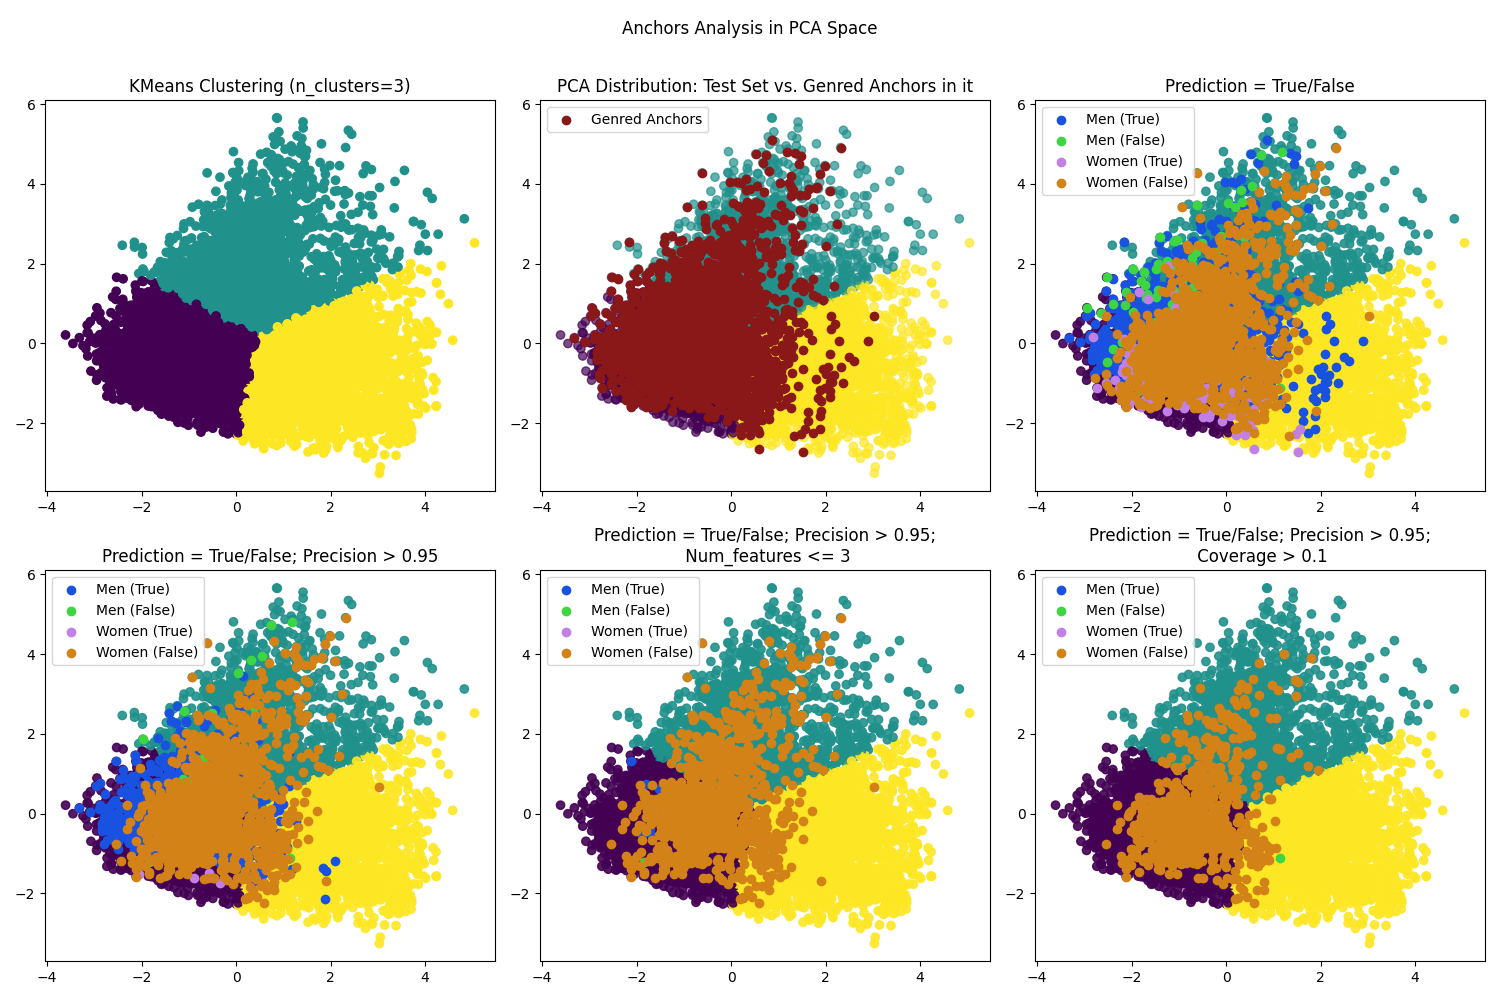
\includegraphics[width=\textwidth]{Images/clustered_pca/clusters_xg_tx_anchors.png}
        \caption{Model: XGBoost, XAI method: Anchors}
        \label{fig:clusters_xg_tx_anchors}
    \end{subfigure}

    \begin{subfigure}[b]{1.0\textwidth}
        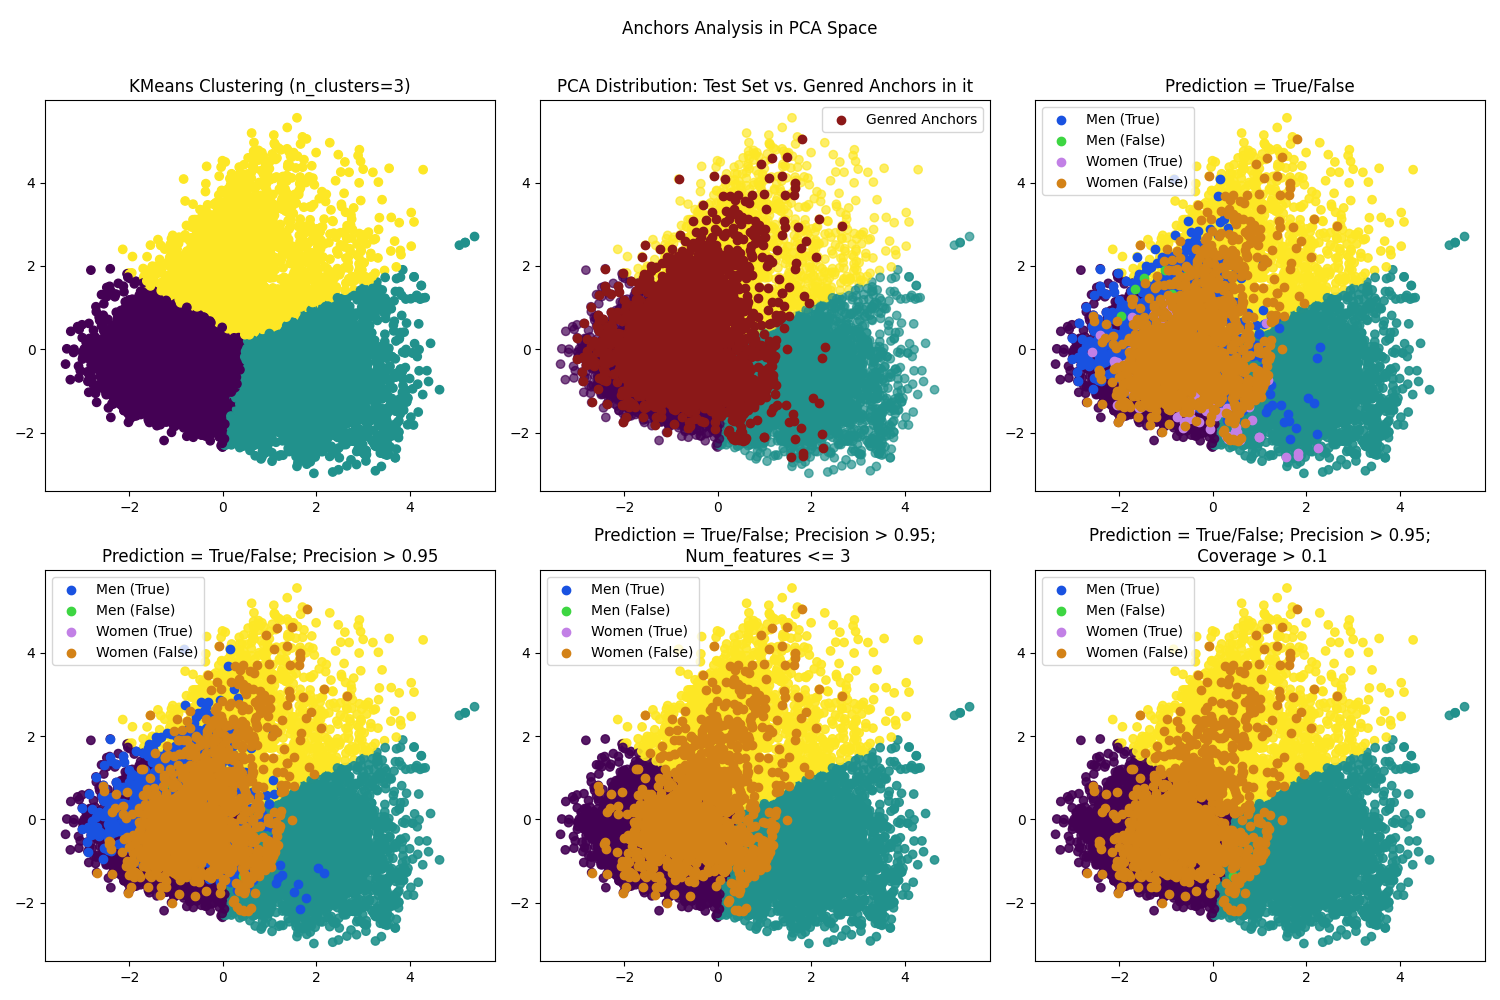
\includegraphics[width=\textwidth]{Images/clustered_pca/clusters_skrub_tx_anchors.png}
        \caption{Model: HistGradientBoosting, XAI method: Anchors}
        \label{fig:clusters_skrub_tx_anchors}
    \end{subfigure}
    \caption{Comparison of the clustered PCA in the Texas state, putting in evidence gendered explanations (Part 1)}
\end{figure}

\begin{figure}[h]
    \ContinuedFloat
    \begin{subfigure}[b]{1.0\textwidth}
        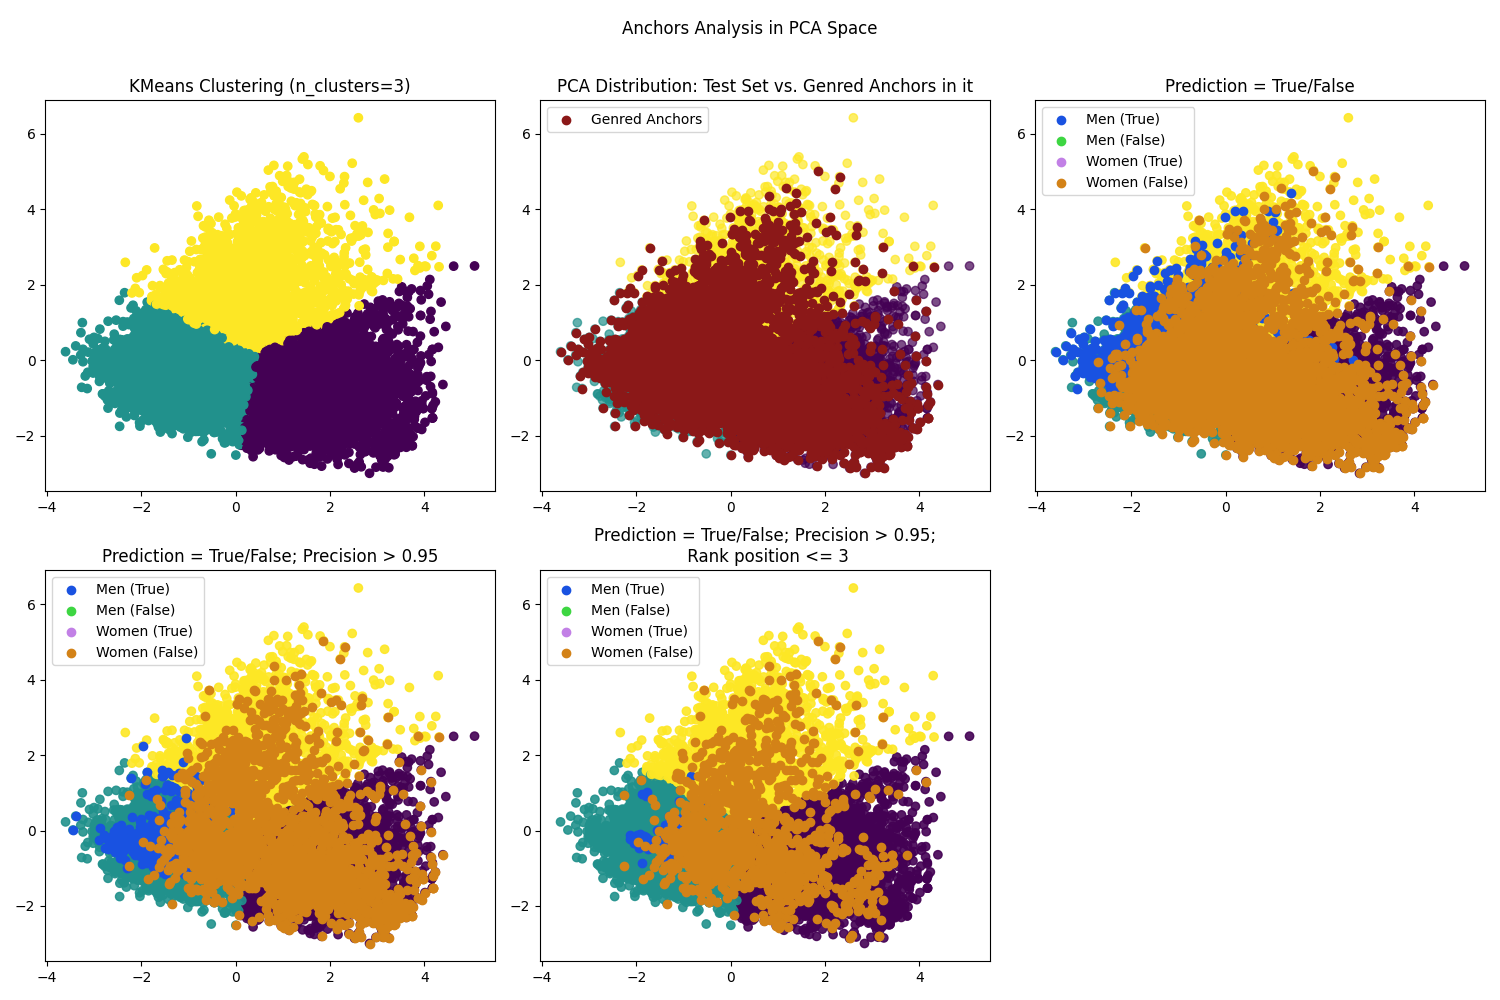
\includegraphics[width=\textwidth]{Images/clustered_pca/clusters_xg_tx_shap.png}
        \caption{Model: XGBoost, XAI method: SHAP}
        \label{fig:clusters_xg_tx_shap}
    \end{subfigure}

    \begin{subfigure}[b]{1.0\textwidth}
        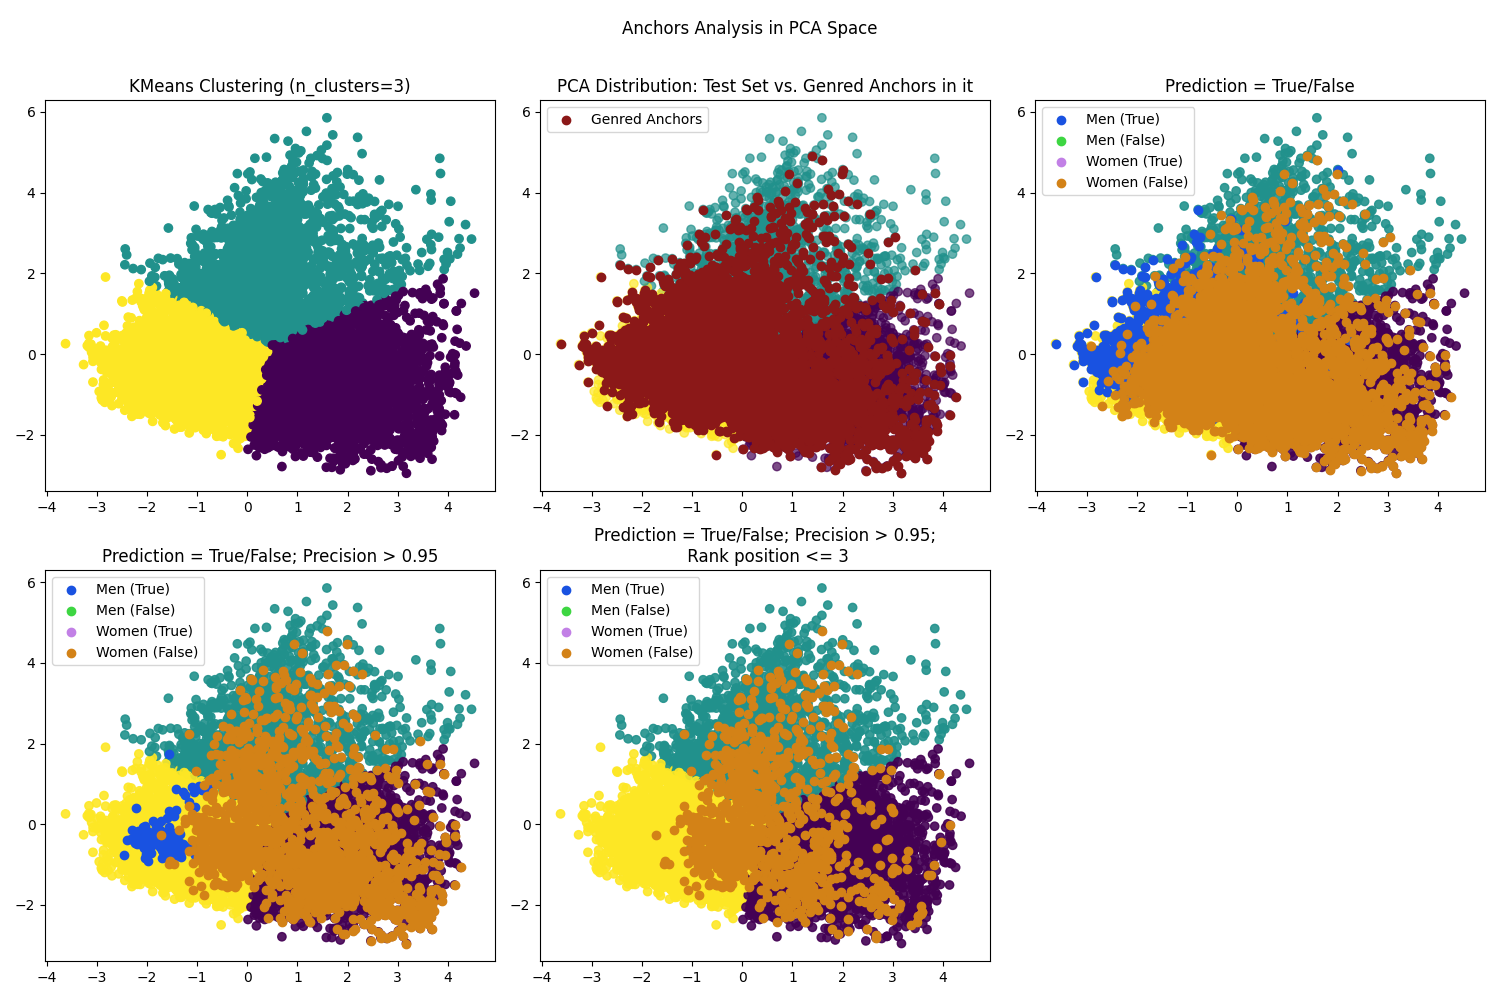
\includegraphics[width=\textwidth]{Images/clustered_pca/clusters_skrub_tx_shap.png}
        \caption{Model: HistGradientBoosting, XAI method: SHAP}
        \label{fig:clusters_skrub_tx_shap}
    \end{subfigure}

    \caption{Comparison of the clustered PCA in the Texas state, putting in evidence gendered explanations (Part 2)}
    \label{fig:clusters_tx}
\end{figure}